%%%%%%%%%%%%%%%%%%%%%%%%%%%%%%%%%%%%%%%%%%%%%%%%%%%
%% P3: Phenomenology of Particle Physics                         
%%
%% Author:  André Rubbia                   		 
%%
%% Figure 11.15 The kinematics for the pair annihilation into two photons in the center-of-mass frame. 
%%
%% This work is licensed under the Creative Commons Attribution 4.0 International License. 
%% To view a copy of this license, visit http://creativecommons.org/licenses/by/4.0/ or 
%% send a letter to Creative Commons, PO Box 1866, Mountain View, CA 94042, USA.
%%
%%%%%%%%%%%%%%%%%%%%%%%%%%%%%%%%%%%%%%%%%%%%%%%%%%%

\documentclass[a4paper,10pt]{article}

\usepackage[T1]{fontenc}
\usepackage[utf8]{inputenc}
\usepackage{lmodern}
\usepackage[labelfont=bf]{caption}
\usepackage{upgreek}

\usepackage{tikz}
\usepackage{pgfplots}
\pgfplotsset{compat=1.17}
\usepgfplotslibrary{ternary}
\usepgfplotslibrary{fillbetween}
\usepgfplotslibrary{external}

\usepackage{braket}

\def\d{\mathrm{d}}

\begin{document}

%%%%%%%%%%%%%%%%% FIGURE %%%%%%%%%%%%%%%%%%%%%%%%%%%%%%%%%%
\begin{figure}[htb]
\begin{center}
\mbox{
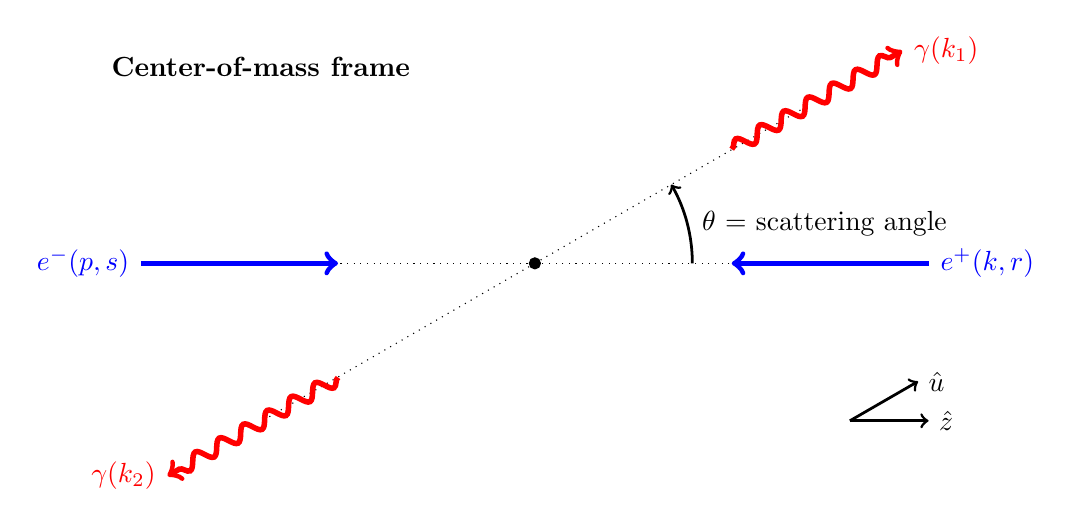
\begin{tikzpicture}
\draw[dotted] (-5,0)  -- (0,0);
\draw[dotted] (5,0)  -- (0,0);
\draw[dotted] (0,0) -- +(30:4);
\draw[dotted] (0,0) -- +(-150:4);
\draw[thick,->,line width=1pt] (2,0) arc [radius=2, start angle =0, end angle=30];
\draw (2,0.5) node[right] {$\theta$ = scattering angle};
\draw[->,line width=1pt] (4,-2) -- (5,-2) node[right] {$\hat z$};
\draw[->,line width=1pt] (4,-2) -- +(30:1) node[right] {$\hat u$};
\draw[->,blue,line width=2pt] (-5,0)  node[left] {$e^-(p,s)$} -- (-2.5,0);
\draw[->,blue,line width=2pt] (5,0)  node[right] {$e^+(k,r)$} -- (2.5,0);
\draw[red,->,decorate, decoration=snake,line width=2pt] (2.5,1.45)  -- +(30:2.5) node[right] {$\gamma(k_1)$};
\draw[red, ->,decorate, decoration=snake,line width=2pt] (-2.5,-1.45)  -- +(-150:2.5) node[left] {$\gamma(k_2)$};
\filldraw [black] (0,0) circle (2pt);
\draw[] (-5.5,2.5) node[right] {\textbf{Center-of-mass frame}};
\end{tikzpicture}
}
\caption{The kinematics for the pair annihilation into two photons in the center-of-mass frame. }
\end{center}
\end{figure}
%%%%%%%%%%%%%%%%% END FIGURE %%%%%%%%%%%%%%%%%%%%%%%%%%%%%%
%

\end{document}
